\section{CHAD at First-Order}
\label{sec:first-order}

\todo{Salvage some of this for \secref{semantic-gps}}

\subsection{First-Order Galois Slicing via CHAD}
\label{sec:fam:galois-slicing}

The total category $\Fam(\LatGal)$ is then a suitable setting for interpreting first-order programs for \GPS.
It has as objects $(X, \partial X)$, all pairs of a set $X$ and and for every $x \in X$, a bounded lattice
$\partial X(x)$, and as morphisms $(X, \partial X) \to (Y, \partial Y)$, all pairs $(f, \partial f)$ of a
function $f: X \to Y$ and for every $x \in X$, a Galois connection $\partial f(x): \partial X(x) \to \partial
Y(f(x))$. The reindexing along $f$ in the composition $(g, \partial g) \comp (f, \partial f) = (g \comp f,
\reindex{\partial g}{f} \comp \partial f)$ selects the appropriate lattice of approximations and Galois
connection at each point, using the baseline (unapproximated) function $f$.

For a first-order language with a primitive type $\syn{nat}$ and primitive operations such as $+$, the
language would provide a model of $\syn{nat}$ and its operations in $\Fam(\LatGal)$. For example, we might
interpret $\syn{nat}$ as the object $(\Nat,n \mapsto \downset{n})$, where the family component assigns to
every natural number $n$ the two-point lattice $\downset{n} = \{n, \bot\}$ indicating whether $n$ is fully
present ($n$) or fully absent ($\bot$) from an approximation of $n$, as shown in the example in
\secref{introduction}. A slight variant is to use the constant family which assigns to every $n$ the two-point
lattice $\Two = \{\mathsf{tt},\mathsf{ff}\}$; using $\downset{n}$ can be more useful in practice as the
approximants of a given value then contain all the information about the value that hasn't been approximated
away.

We might interpret $+$ as the morphism $(+,\partial+)$, i.e.~the usual addition operator + paired with an
approximating version $\partial+_{n,m}: \downset{n} \to \downset{m}$ defined as:
\begin{displaymath}
    \begin{array}[t]{l@{(}l@{,~}l@{)~}c@{~}l}
      \partial+_{n,m}&n&m&=&n + m \\
      \partial+_{n,m}&\bot&\_&=&\bot \\
      \partial+_{n,m}&\_&\bot&=&\bot
    \end{array}
\end{displaymath}
These elementary approximation structures would then be combined by the interpretation of composite types like
sums and products, providing suitable derived structures for composite values.

\subsubsection{Lifting}

A programmer (or perhaps language implementor) might want to embed additional ``approximation points'' into
composite data types, to allow for richer approximation structures. For example, for a list like $1 : 2 : []$
we might want to allow the partial lists $\bot$, $1 : \bot$ and $1 : 2 : \bot$ as approximants, in addition to
the approximants obtained by replacing elements with $\bot$. This can be accomplished by extending the syntax
with a \emph{lifting} type constructor $\tyLift$. Then, as an alternative to the usual definition of lists of
natural numbers as $\mu\alpha.1 + \synVar{nat} \times \alpha$, one could (within the language) define a type
of ``approximation lists'' $\mu\alpha.\tyLift\,(1 + \tyLift\,\synVar{nat} \times \alpha)$, with monadic
computations over approximated lists computing partial lists like $1 : \bot$. The lattice of approximants of
$1 : 2 : []$ now includes not only all ``shape-preserving'' approximations but also all prefixes obtained by
truncating successive tails with $\bot$:

  \begin{center}
    \tikzset{node distance=1cm}
    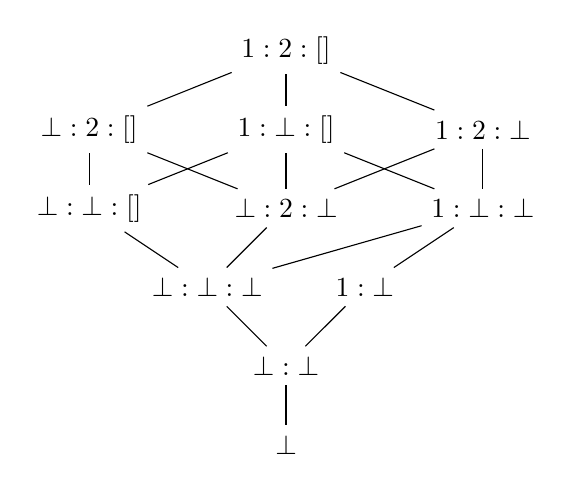
\begin{tikzpicture}
      \node (top) at (0,0) {$1 : 2 : []$};
      % row 2
      \node [below of=top] (ioi) {$1 : \bot : []$};
      \node [left of=ioi,xshift=-1.5cm] (oii) {$\bot : 2 : []$};
      \node [right of=ioi,xshift=1.5cm] (iio) {$1 : 2 : \bot$};
      % row 3
      \node [below of=ioi] (oio) {$\bot : 2 : \bot$};
      \node [left of=oio,xshift=-1.5cm] (ooi) {$\bot : \bot : []$};
      \node [right of=oio,xshift=1.5cm] (ioo) {$1 : \bot : \bot$};
      % row 4
      \node [below of=oio,xshift=-1cm] (ooo) {$\bot : \bot : \bot$};
      \node [below of=oio,xshift=1cm] (io) {$1 : \bot$};
      % row 5
      \node [below of=ooo,xshift=1cm] (oo) {$\bot : \bot$};
      % row 6
      \node [below of=oo] (o) {$\bot$};

      % links
      \draw (top) -- (ioi);
      \draw (top) -- (oii);
      \draw (top) -- (iio);
      \draw (ioi) -- (oio);
      \draw (ioi) -- (ooi);
      \draw (ioi) -- (ioo);
      \draw (oii) -- (oio);
      \draw (oii) -- (ooi);
      \draw (iio) -- (oio);
      \draw (iio) -- (ioo);
      \draw (ooi) -- (ooo);
      \draw (oio) -- (ooo);
      \draw (ioo) -- (ooo);
      \draw (ioo) -- (io);
      \draw (ooo) -- (oo);
      \draw (io) -- (oo);
      \draw (oo) -- (o);
    \end{tikzpicture}
  \end{center}

Similarly, one could define a custom approximating version of multiplication $*_{\text{appr}}:
\tyLift\,\synVar{nat} \times \tyLift\,\synVar{nat} \to \tyLift\,\synVar{nat}$, as:
\[x *_{\text{appr}} y = \tmBind{x}{\tmFun{x'}{\syn{if}\;x' \equiv
0\;\syn{then}\;\tmReturn{0}\;\syn{else}\;\tmBind{y}{\tmFun{y'}{\tmReturn{x' * y'}}}}}\]

\noindent This would allow the programmer to emulate the short-circuiting behaviour of $\mathrm{strictOr}$
from \exref{strict-short-circuit}, or the short-circuiting multiplication used in \citet{perera22} for slicing
matrix convolutions, without having to bake specific choices of approximation into the interpretation of
individual operators.

With this lifting operator in the core language, one could then choose to fix certain choices of
approximation, providing a surface language without the lifting monad and interpreting it into the core
language with lifting. The Galois slicing implementations discussed in \citet{perera12a} and
\citet{ricciotti17}, for example, provide an approximation point at every composite type constructor; we can
emulate this in our approach by defining a surface language where the data type of lists $\mu\alpha.1 +
\synVar{nat} \times \alpha$ desugars automatically into the approximating version $\mu\alpha.\tyLift\,(1 +
\tyLift\,\synVar{nat} \times \alpha)$.

To interpret the syntactic type constructor $\tyLift$, consider the strong monad $(\Lift, \eta, \mu)$ which
acts on a poset $X$ to extend it with a distinguished bottom element $\bot$ and on a monotone function $f$
between posets to extend it with a mapping from $\bot$ to $\bot$. $\Lift$ is also a strong monad on
meet-semilattices. On (bounded) join-semilattices, $\Lift$ induces a costrong comonad $(\Lift, \varepsilon,
\delta)$, with the bottom element of $X$ needed to implement the counit $\varepsilon_X: \Lift(X) \to X$. These
two combine to form a strong lifting monad in $\LatGal$ with unit $\varepsilon_X \dashv \eta_X$ and
multiplication $\delta_X \dashv \mu_X$.

The lifting monad $\Lift$ in $\LatGal$ is preserved into $\Fam(\LatGal)$. The families construction, regarded
as a covariant 2-functor $\Fam(-): \Cat \to \Cat$, sends functors $F: \cat{C} \to \cat{D}$ to functors
$\Fam(F): \Fam(\cat{C}) \to \Fam(\cat{D})$ that reassign the target category by postcomposing with $F$,
sending objects $(X, \partial X)$ to $(X, F \comp \partial X)$ and morphisms $(f, \partial f)$ to $(f, F \comp
\partial f)$, where $F \comp \partial f$ denotes the natural transformation where $(F \comp \partial f)(x) =
F(\partial f(x))$. If $F$ happens to be a (strong) monad on $\cat{C}$, then $\Fam(F)$ is a (strong) monad on
$\Fam(\cat{C})$, computed by extending the original monad $F: \cat{C} \to \cat{C}$ componentwise to families.
